\section{Iris Recognition}
\label{sec:Iris_Recognition_Research}
Modern iris recognition started in with an article by \cite{Daugman1993} discussing the security of using iris for recognition. Here an outline of how to do recognition was also laid out with the introduction of using  2D Gabor Waveletts to extract features of the complex pattern that can be found in an iris. The field has been developted extensivly since then but the general methodology is more or less the same. A modern system is typically composed of image acquisition, segmentation, normalization, feature extraction and matching. 

\subsection{Images}
The images aquired are often taken in the Near Infra-Red (NIR) spectrum which is ranging between 700 nm and 900 nm i wavelength. In this band the melanin in the iris, which is the part that gives the iris it's colour e.g. brown or blue, is typically negligible making the unique patterns in the iris very distinct. To acquire usable NIR images the user has to be in the milimeter range of the NIR camera.  In the visible light the melanin is seen much more clearly and thus makes is harder to detect the patters. The abbreviation for visible light is not agreed upon in the literature with some examples being Visible Light (VL) , Visible Spectrum (VIS), and Visible Wavelength (VW). It will be abbreviated VL \fxnote{needs to be agreed on} in this report. On the other hand other useful features can be seen in the VL that cannot be seen with NIR. These can include the moles, freckles and conjunctival vasculature which can help in making more accurate recognition systems. To make iris recognitions systems comparable with each other some publicaly available databases are often used. \cite{RifaeeMustafaandAbdallahMohammadandOkosh2017}  give an outline of the some of the free databases that are used in research. A comprehensive table depicting the databases and their contents, sample image and type of noise can be found in \autoref{fig:Iris_database_1} and \autoref{fig:Iris_database_2}. Most of the databases available are NIR images with CASIA being one of the most used database. For VL images UBIRIS in the most common used.  These contain more "real world" data as the images contain more noise in the form of eyelids obstruction, eyelash obstruction, glare, motion blur, out-of-focus or poor focused iris, partial iris and specular reflection \citep{Rattani2017}. The database has also been used in Noisy Iris Challenge Evaluation (NICE) I. The increasing usage of mobile devices also proposes an opportunity to integrate iris recognition as a biometric for verifying the user.  For this purpose a competition, Mobile Iris CHallenge Evaluation (MICHE), is made to compare the state of the art mobile iris. They provide a the MICHE database that can be used which they claim is a better database than UBRIS for mobile systems. The database contains noisy iris images taken with a Galaxy Samsung IV, Iphone5 and Galaxy Tablet II. The noise includes noise from both artificial and natural light sources during acquisition, motion blur, occlusion due to eyelids/glasses/eyelashes/hair/shadows which can naturally occur when a user is trying to unlock a phone using their iris. 

\subsection{Segmentation}





%\cite{RifaeeMustafaandAbdallahMohammadandOkosh2017} gives an outline of commercially free databases often used in research.\autoref{fig:Iris_database_1} and \autoref{fig:Iris_database_2} show the different contents of the databases. Most of the databases are NIR images with CASIA being one most used databases in the literature.  For images in the visible light UBRIS is often used . These contain more "real world" data as the images contain more noise in the form of eyelids obstruction, eyelash obstruction, glare, motion blur, out-of-focus or poor focused iris, partial iris and spec- ular reflection \citep{Rattani2017}. The database has also been used in Noisy Iris Challenge Evaluation (NICE) I. For iris recognition system on mobile platforms the Mobile Iris CHallenge Evaluation (MICHE) database can be used.  The database contains noisy images taken withe Galaxy Samsung IV, Iphone5 and Galaxy Tablet II. The noise includes noise from both artificial and natural light sources during acquisition, motion blur, occlusion due to eyelids/glasses/eyelashes/hair/shadows which can naturally occur when a user is trying to unlock a phone using their iris. 


. It was also the foundation for IrisCode which is a commercially developed iris recognition algorithm by John Daugman. In 2016 a handbook for iris recognition by \cite{Bowyer2016b} was published giving an outline of the whole process of iris recognition. In general Near Infra-Red (NIR) images of an iris are used but other type of images can also be used.  \cite{Khan2017a} show how to use Daugmans methodology on iris images taken with a smartphone in visible light. They use Daugmans Integro-differential operator to localise the bounds of the iris. Then they suppress the eyelids the eyelids which often cover parts of the iris by using an approach inspired by Masek. Afterwards the image is normalised by using the homogeneous rubber sheet model by Daugman. Then eyelashes are removed from the image and feature extraction is done by using 2D Gabor Waveletts. This approach to extract features in one way or another can be seen in multiple state of the art iris recognition systems and research papers e.g \citep{Luhadiya2017a,Uka2017a,Kuehlkamp2016a}, \cite{Kuehlkamp2016a}. After the features have been extracted they are compared/categorised. Traditionally a "1-to-N search" has been done. Here the Hamming distance of features of the scanned iris are compared to the whole database and it is classified with the iris that has the least distance. \cite{Kuehlkamp2016a} have suggested using a "1-to-first search" instead to improve the speed of the search. Here a threshold is chosen and as soon as a match has been found below the threshold it will stop the search. Other approaches to the categorisation have been proposed using machine learning. \cite{Khan2017a} proposed using Support Vector Machines (SVM), K-Nearest-Neighbours(KNN) and Linear Discriminant Analysis (LDA) with respective test accuracies of 97\%, 95.1\%, 94.28\%. \cite{Zhao2017b} proposed using deep learning to classify. They claim that research in neural networks with iris recognition is still very new and not much has been done. But some of the work that has been done have used Convolutional Neural Networks (CNN) and a Deep Belief Network (DBN). They claim that the problem with traditional networks are that they are very database specific on not very generalisable. \cite{Zhao2017b} created a Fully Convolutional Network (FCN) using a loss function they created specifically for iris networks called Extended Triplet Loss (ETL). They claim this network is more generalisable than the previous networks. 



\begin{figure}
\centering
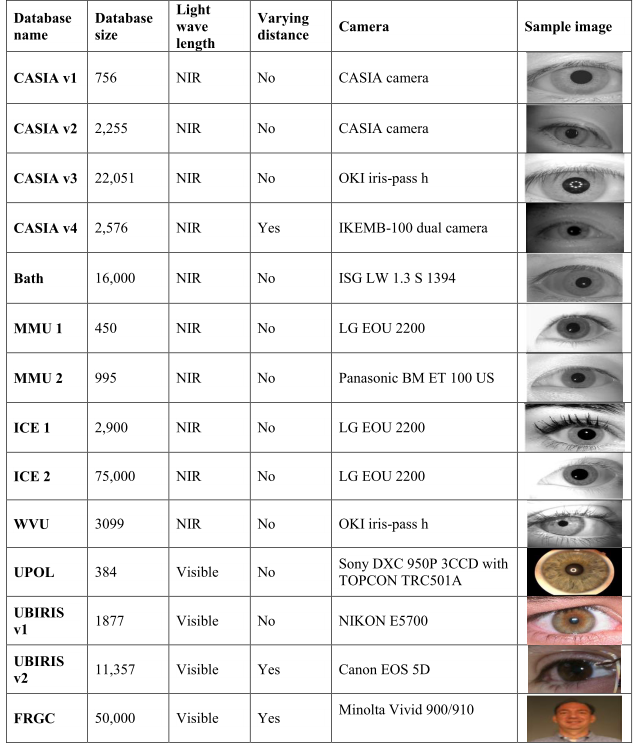
\includegraphics[width=\textwidth]{figures/Iris_Database_tabel_1.png} 
\caption{A table depicting the contents of free iris image databases.}
\label{fig:Iris_database_1}
\end{figure}

\begin{figure}
\centering
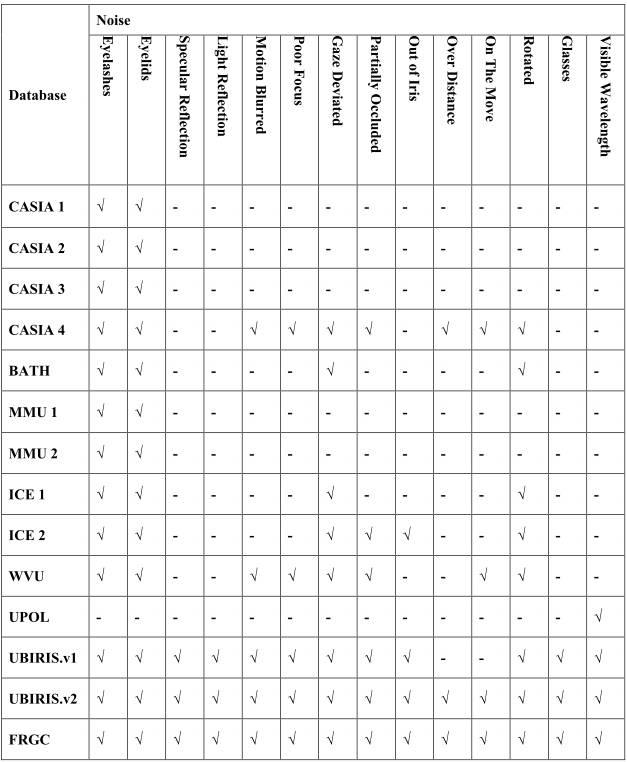
\includegraphics[width=\textwidth]{figures/Iris_Database_tabel_2.png} 
\caption{A table depicting the noise present in the databases}
\label{fig:Iris_database_2}
\end{figure}

